% Provenance (never printed): see sources/outline_sources.md (Year 3: the
% Rayleigh number; thermal boundary layers; slab pull and ridge push; plumes;
% post-glacial rebound and mantle viscosity). Brief: sources/book5/BRIEFS.md,
% ch. 6. Curves from figdata/bachelor-3/convection_scaling.py (PREM read only),
% gia_relaxation.py and ridge_push.py (on plate_cooling.py). Exercise and
% problem values in the Book 5 scratch calculator calc/ch06.py.
\chapter{Convecção no manto e forças motrizes das placas}\label{ch:b3:mantle-convection}

A costa do norte da Suécia emerge do mar à taxa de cerca de um centímetro por
ano, dez mil anos depois que a capa de gelo que a cobria derreteu; as
margens da baía de Hudson sobem com a mesma rapidez. Nada as empurra para
cima a não ser o manto, que flui lentamente de volta sob o local que o gelo
havia comprimido. A taxa com que o solo se recupera mede a \omterm{def:b3:mantle-convection:gia}{viscosidade do manto},
e essa mesma viscosidade determina a rapidez com que o manto convecta e as
placas se movem. Este capítulo pergunta por que o manto sólido convecta, com
que velocidade ele precisa fluir para transportar o calor da Terra, quais forças
movem as placas e o que a recuperação do solo revela sobre a \omterm{def:b3:mantle-convection:gia}{viscosidade do manto}.
% ledger: vestol19:umea, zhao12:fenno, sella07:gia

\begin{recall}
A viscosidade, o escoamento lento de um fluido viscoso (as equações de Stokes
$\nabla p = \eta\nabla^2\mathbf u$, $\nabla\cdot\mathbf u = 0$), a lei de Stokes
para uma esfera, o número de Reynolds e a flutuabilidade estão nos volumes de
física universitários. A convecção no manto e o rebote isostático foram
vistos no volume do ensino médio (12º ano), e o empurrão da dorsal e a tração da laje na parte do 11º ano.
A camada limite térmica, a litosfera térmica e a adiabática do manto estão no
volume do primeiro ano, no capítulo sobre o balanço de calor da Terra; pontos
quentes, plumas do manto e grandes províncias ígneas estão no capítulo sobre
pontos quentes. O \omterm{def:b3:lithosphere-thermal-models:half-space}{modelo de resfriamento do semiespaço} está no \cref{ch:b3:lithosphere-thermal-models},
a flexura da litosfera no \cref{ch:b3:gravity-geodesy}, e a
\omterm{def:b3:seismology-imaging:tomography}{tomografia sísmica} no \cref{ch:b3:seismology-imaging}.
\end{recall}

\section{Por que o manto convecta}

O manto é sólido: ele transmite ondas S. Ao longo de milhões de anos, porém,
ele flui lentamente como um fluido de viscosidade enorme, e uma camada de
fluido aquecida por baixo e resfriada por cima pode permanecer em repouso, com
o calor atravessando-a por condução, ou pode se revirar. Uma porção de fluido
quente de tamanho $d$, mais leve que o entorno em $\rho\alpha\,\Delta T$, sobe
com velocidade da ordem de $\rho g\alpha\,\Delta T d^2/\eta$; ela perde seu calor
por difusão em um tempo da ordem de $d^2/\kappa$. Se ela puder subir através da
camada antes de ter esfriado, a camada se revira.

\begin{definition}[Número de Rayleigh]\label{def:b3:mantle-convection:rayleigh}
Para uma camada de fluido de espessura $d$, densidade $\rho$, coeficiente de
expansão térmica $\alpha$, difusividade térmica $\kappa$ e viscosidade $\eta$,
sob a gravidade $g$, com uma diferença de temperatura $\Delta T$ entre sua base
e seu topo, o \emph{número de Rayleigh}\index{número de Rayleigh} é
\[
  \mathrm{Ra} = \frac{\rho g\alpha\,\Delta T d^3}{\kappa\eta},
\]
a razão entre o tempo de difusão $d^2/\kappa$ e o tempo de ascensão por
flutuabilidade $\eta/(\rho g\alpha\,\Delta Td)$.
\end{definition}

\begin{definition}[Número de Rayleigh crítico]\label{def:b3:mantle-convection:critical}
O \emph{número de Rayleigh crítico}\index{número de Rayleigh crítico}
$\mathrm{Ra}_c$ de uma camada é o valor do \omterm{def:b3:mantle-convection:rayleigh}{número de Rayleigh} acima do qual uma
pequena perturbação do estado de repouso cresce até tornar-se convecção, e abaixo
do qual ela se extingue.
\end{definition}

\begin{proposition}[Início da convecção]\label{prop:b3:mantle-convection:onset}
Para uma camada cujos topo e base estão livres de tensão de cisalhamento e
mantidos a temperaturas fixas, uma perturbação de número de onda horizontal $k$
(em unidades de $1/d$) cresce quando $\mathrm{Ra} > (\pi^2 + k^2)^3/k^2$. O mínimo do
lado direito, em $k = \pi/\sqrt2$, fornece
\[
  \mathrm{Ra}_c = \frac{27\pi^4}{4} \approx 657.5,
\]
e as primeiras células a aparecer têm largura $2\sqrt2\,d$. Entre contornos rígidos,
$\mathrm{Ra}_c \approx 1708$.
\end{proposition}

\admitted
A análise de estabilidade linear que o sustenta, uma perturbação das equações
de calor e de Stokes em torno do estado condutivo, está no tratamento da
convecção nos volumes de física; o exercício 11 verifica o mínimo.

A figura abaixo mostra a camada em convecção. Os valores do manto, com a
profundidade do limite manto--núcleo, $d = \qty{2891}{km}$, a densidade média do
manto, \qty{4476}{kg.m^{-3}}, e $g$ entre 9.8 e
\qty{10.7}{m.s^{-2}}, todos do modelo sísmico da Terra PREM; $\alpha =
\qty{3.1e-5}{K^{-1}}$ e $\Delta T = \qty{1450}{K}$ do modelo de placa do
\cref{ch:b3:lithosphere-thermal-models}; $\kappa = \qty{e-6}{m^2.s^{-1}}$;
e $\eta$ entre \num{e21} e \qty{e22}{Pa.s} (\cref{sec:b3:mantle-convection:gia}),
dão $\mathrm{Ra}$ entre \num{4.9e6} e \num{4.9e7}, de cerca de sete mil a
setenta mil vezes o crítico. O manto não tem como deixar de convectar.
% ledger: data:prem, honda04:gdh1, delaney86:properties, mitrovica96:haskell, milne04:bifrost

\begin{omfigure}
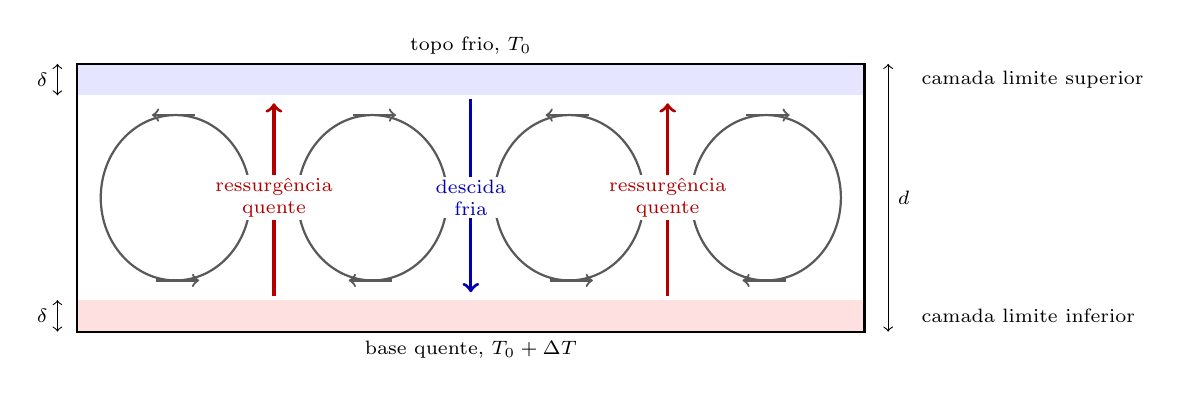
\begin{tikzpicture}[font=\scriptsize, x=1cm, y=1cm]
\fill[blue!10] (0,3.4) rectangle (10,3.0);
\fill[red!12] (0,0) rectangle (10,0.4);
\draw[thick] (0,0) rectangle (10,3.4);
\node[above] at (5,3.4) {topo frio, $T_0$};
\node[below] at (5,0) {base quente, $T_0 + \Delta T$};
\foreach \c/\s in {1.25/1, 3.75/-1, 6.25/1, 8.75/-1} {
  \draw[gray!70!black, thick] (\c,1.7) ellipse[x radius=0.95, y radius=1.05];
  \draw[->, gray!70!black, thick] ({\c+0.25*\s},2.75) -- ({\c-0.3*\s},2.75);
  \draw[->, gray!70!black, thick] ({\c-0.25*\s},0.65) -- ({\c+0.3*\s},0.65);
}
\draw[->, red!70!black, very thick] (2.5,0.45) -- (2.5,2.9);
\draw[->, red!70!black, very thick] (7.5,0.45) -- (7.5,2.9);
\draw[->, blue!70!black, very thick] (5,2.95) -- (5,0.5);
\node[red!70!black, fill=white, inner sep=1pt, align=center] at (2.5,1.7) {ressurgência\\quente};
\node[red!70!black, fill=white, inner sep=1pt, align=center] at (7.5,1.7) {ressurgência\\quente};
\node[blue!70!black, fill=white, inner sep=1pt, align=center] at (5,1.7) {descida\\fria};
\draw[<->] (10.3,0) -- (10.3,3.4) node[midway, right] {$d$};
\draw[<->] (-0.25,3.0) -- (-0.25,3.4) node[midway, left] {$\delta$};
\draw[<->] (-0.25,0) -- (-0.25,0.4) node[midway, left] {$\delta$};
\node[anchor=west] at (10.6,3.2) {camada limite superior};
\node[anchor=west] at (10.6,0.2) {camada limite inferior};
\end{tikzpicture}

\par\smallskip{\small Convecção em uma camada aquecida por baixo e resfriada por
cima. O calor atravessa as finas camadas limite, de espessura $\delta$, por
condução; entre elas, o interior bem misturado o transporta por escoamento. Placas frias
se destacam da camada superior e afundam; as quentes sobem a
partir da inferior.}\label{fig:b3:mantle-convection:cell}
\end{omfigure}

O manto também é aquecido por dentro, pelo decaimento de elementos radioativos,
e por baixo, pelo núcleo. Uma camada aquecida apenas por dentro não tem
camada limite quente em sua base: seu escoamento é impulsionado por placas frias que afundam do
topo, sendo o escoamento ascendente um retorno amplo e passivo. As lajes são essas placas, e
as plumas necessitam do calor do núcleo.

\section{Camadas limite e a intensidade da convecção}

\begin{definition}[Número de Nusselt]\label{def:b3:mantle-convection:nusselt}
O \emph{número de Nusselt}\index{número de Nusselt} de uma camada em convecção é o
fluxo de calor através dela dividido pelo fluxo de calor que a condução, sozinha, transportaria
através da mesma camada, $\mathrm{Nu} = q\,d/(k\,\Delta T)$.
\end{definition}

\begin{theorem}[Escala de camada limite da convecção]\label{thm:b3:mantle-convection:scaling}
Em uma camada em convecção com $\mathrm{Ra} \gg \mathrm{Ra}_c$, se cada camada limite térmica
cresce até que seu próprio \omterm{def:b3:mantle-convection:rayleigh}{número de Rayleigh}, construído com sua espessura
$\delta$ e com a queda de temperatura $\Delta T/2$ através dela, atinja
$\mathrm{Ra}_c$, então
\[
  \delta = d\Bigl(\frac{2\mathrm{Ra}_c}{\mathrm{Ra}}\Bigr)^{1/3},\qquad
  \mathrm{Nu} = \frac12\Bigl(\frac{\mathrm{Ra}}{2\mathrm{Ra}_c}\Bigr)^{1/3},
  \qquad
  u = \frac\kappa d\Bigl(\frac{\mathrm{Ra}}{2\mathrm{Ra}_c}\Bigr)^{2/3},
\]
em que $u$ é a escala de velocidade do escoamento, definida exigindo que a
camada cresça até $\delta$ enquanto o fluido atravessa a célula. Esta é a
\emph{escala de camada limite da convecção}\index{escala de camada limite da convecção}.
\end{theorem}

\begin{proof}
O interior é bem misturado, à temperatura média, de modo que cada camada limite
carrega metade de $\Delta T$. Seu \omterm{def:b3:mantle-convection:rayleigh}{número de Rayleigh} é $\rho g\alpha(\Delta T/2)
\delta^3/(\kappa\eta) = \mathrm{Ra}\,(\delta/d)^3/2$; igualando-o a
$\mathrm{Ra}_c$ obtém-se $\delta$. O fluxo de calor é conduzido através da camada,
$q = k(\Delta T/2)/\delta$, de modo que $\mathrm{Nu} = qd/(k\Delta T) = d/(2\delta)$.
Uma camada limite cresce por difusão até a espessura $\delta$ em um tempo
$\delta^2/\kappa$; o fluido do topo atravessa a célula, de largura da ordem de
$d$, em um tempo $d/u$. Igualando os dois tempos, $u = \kappa d/\delta^2 =
(\kappa/d)(d/\delta)^2$.
\end{proof}

O fluxo de calor cresce apenas como a raiz cúbica de $\mathrm{Ra}$: uma viscosidade cem vezes
menor, menos de cinco vezes mais calor. Com o
$\mathrm{Ra} = \num{4.9e7}$ do manto, a escala fornece $\delta \approx \qty{87}{km}$,
$\mathrm{Nu} \approx 17$, um fluxo de calor de $\mathrm{Nu}\,k\Delta T/d \approx
\qty{26}{mW.m^{-2}}$ com $k = \qty{3.1}{W.m^{-1}.K^{-1}}$, e $u \approx
\qty{1.2}{cm/yr}$ (figura abaixo). A camada limite é tão espessa quanto a
placa oceânica do \cref{ch:b3:lithosphere-thermal-models}, \qty{95}{km}; as
velocidades quadráticas médias das placas atuais variam de \qty{1.1}{cm/yr} (América
do Sul) a \qty{7.5}{cm/yr} (Cocos), e \qty{4.4}{cm/yr} para a litosfera inteira. O
fluxo de calor médio da Terra, \qty{92}{mW.m^{-2}}, é de três a quatro
vezes o previsto pela escala: o calor produzido no interior do manto, que uma camada
aquecida por baixo deixa de fora, e as constantes de ordem um que a escala
ignora, ambos pesam. Para uma lei com uma única entrada, as ordens de grandeza
estão corretas: as placas são a camada limite superior de um manto com $\mathrm{Ra}
\sim 10^7$.
% ledger: nnr56:rms, b2dd10:continents, honda04:gdh1

\begin{omfigure}
\begin{tikzpicture}
\begin{groupplot}[group style={group size=1 by 2, vertical sep=2.5cm},
  omrecord, width=0.86\linewidth, height=0.40\linewidth, xmode=log, ymode=log,
  xmin=100, xmax=1e10, xlabel={Número de Rayleigh $\mathrm{Ra}$}]
\nextgroupplot[ylabel={Número de Nusselt}, ymin=0.3, ymax=300,
  title={(a) fluxo de calor, em unidades do fluxo condutivo}, title style={font=\small}]
% computed in figdata/bachelor-3/convection_scaling.py; ledger: data:prem, honda04:gdh1
\addplot[omDef, thick] table[x=ra, y=nu] {figdata/out/bachelor-3-convection_scaling-conduction.dat};
\addplot[red!70!black, thick] table[x=ra, y=nu] {figdata/out/bachelor-3-convection_scaling-scaling.dat};
\addplot[gray, densely dashed, unbounded coords=jump] table[x=ra, y=y] {figdata/out/bachelor-3-convection_scaling-band.dat};
\draw[gray, densely dotted] (axis cs:657.5,0.3) -- (axis cs:657.5,1);
\node[font=\scriptsize, anchor=west] at (axis cs:700,0.45) {$\mathrm{Ra}_c$};
\node[font=\scriptsize, anchor=south west, omDef] at (axis cs:115,1.08) {condução};
\node[font=\scriptsize, anchor=north west, red!70!black] at (axis cs:3e4,0.95) {$\tfrac12(\mathrm{Ra}/2\mathrm{Ra}_c)^{1/3}$};
\node[font=\scriptsize, fill=white, inner sep=1pt] at (axis cs:1.55e7,120) {manto};
\nextgroupplot[ylabel={velocidade (\unit{cm/yr})}, ymin=1e-3, ymax=100,
  title={(b) escala de velocidade para $d = \qty{2891}{km}$}, title style={font=\small}]
\addplot[red!70!black, thick] table[x=ra, y=u] {figdata/out/bachelor-3-convection_scaling-scaling.dat};
\addplot[gray, densely dashed, unbounded coords=jump] table[x=ra, y=y] {figdata/out/bachelor-3-convection_scaling-band.dat};
\addplot[blue!70, thick, dash dot, unbounded coords=jump] table[x=ra, y=u] {figdata/out/bachelor-3-convection_scaling-plates.dat};
\node[font=\scriptsize, anchor=south west, blue!60!black] at (axis cs:150,7.6) {placa mais rápida};
\node[font=\scriptsize, anchor=north west, blue!60!black] at (axis cs:150,1.0) {placa mais lenta};
\node[font=\scriptsize, fill=white, inner sep=1pt] at (axis cs:1.55e7,0.004) {manto};
\end{groupplot}
\end{tikzpicture}

\par\smallskip{\small Escala de convecção. (a) Abaixo de $\mathrm{Ra}_c$ a camada
conduz ($\mathrm{Nu} = 1$); bem acima dela, a lei de camada limite, traçada
a partir de $\mathrm{Ra} = 16\,\mathrm{Ra}_c \approx \num{1.1e4}$, onde fornece $\mathrm{Nu} = 1$ (entre esses valores,
a convecção se instala gradualmente). (b) A escala de velocidade
para a profundidade do manto e $\kappa = \qty{e-6}{m^2.s^{-1}}$, com a
faixa das velocidades atuais das placas (traço e ponto). As linhas tracejadas delimitam o
\omterm{def:b3:mantle-convection:rayleigh}{número de Rayleigh} do manto para viscosidades de \num{e22} e \qty{e21}{Pa.s}.}\label{fig:b3:mantle-convection:scaling}
\end{omfigure}

\section{As forças sobre uma placa}

Uma placa se move a uma velocidade constante: as forças sobre ela se equilibram. Três delas a impulsionam ou
a resistem por suas bordas e sua base (figura abaixo). A força que a
laje em afundamento exerce sobre sua placa, a tração da laje, provém do excesso de
densidade de uma laje fria no manto mais quente. O empurrão da dorsal, o empuxo da dorsal alta e quente
sobre a placa mais fria ao lado, decorre do modelo de semiespaço
apresentado no \cref{ch:b3:lithosphere-thermal-models}.

\begin{omfigure}
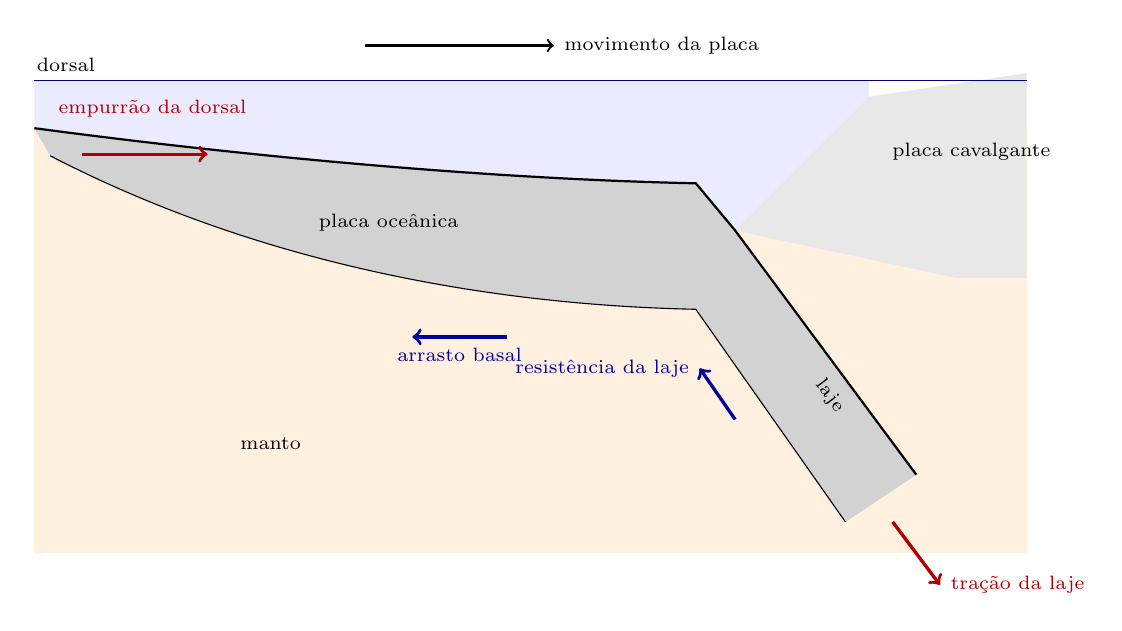
\begin{tikzpicture}[font=\scriptsize, x=1cm, y=1cm]
\fill[orange!12] (0,-0.6) rectangle (12.6,-6.0);
\fill[blue!8] (0,0) -- (0,-0.6) .. controls (3,-1.0) and (6,-1.25) .. (8.4,-1.3) -- (8.9,-1.9) -- (10.6,-0.2) -- (10.6,0) -- cycle;
\fill[gray!35] (0,-0.6) .. controls (3,-1.0) and (6,-1.25) .. (8.4,-1.3) -- (8.9,-1.9) -- (11.2,-5.0) -- (10.3,-5.6) -- (8.4,-2.9) .. controls (6,-2.85) and (3,-2.4) .. (0.2,-0.95) -- cycle;
\fill[gray!18] (10.6,-0.2) -- (12.6,0.1) -- (12.6,-2.5) -- (11.7,-2.5) -- (8.9,-1.9) -- cycle;
\draw[thick] (0,-0.6) .. controls (3,-1.0) and (6,-1.25) .. (8.4,-1.3) -- (8.9,-1.9) -- (11.2,-5.0);
\draw (0.2,-0.95) .. controls (3,-2.4) and (6,-2.85) .. (8.4,-2.9) -- (10.3,-5.6);
\draw[blue!50!black] (0,0) -- (12.6,0);
\node at (0.4,0.2) {dorsal};
\node at (4.5,-1.8) {placa oceânica};
\node at (11.9,-0.9) {placa cavalgante};
\node[rotate=-53] at (10.1,-4.0) {laje};
\node at (3,-4.6) {manto};
\draw[->, very thick, red!70!black] (0.6,-0.93) -- (2.2,-0.93);
\node[red!70!black] at (1.5,-0.35) {empurrão da dorsal};
\draw[->, very thick, red!70!black] (10.9,-5.6) -- (11.5,-6.4) node[right] {tração da laje};
\draw[->, very thick, blue!60!black] (6.0,-3.25) -- (4.8,-3.25) node[below, pos=0.5] {arrasto basal};
\draw[->, very thick, blue!60!black] (8.9,-4.3) -- (8.45,-3.65) node[left] {resistência da laje};
\draw[->, thick] (4.2,0.45) -- (6.6,0.45) node[right] {movimento da placa};
\end{tikzpicture}

\par\smallskip{\small As forças sobre uma placa oceânica: o empurrão da dorsal e a tração da laje
a impulsionam (vermelho); o arrasto na base, onde a placa se move mais depressa que o manto
abaixo, e a resistência viscosa do manto à laje em afundamento a resistem
(azul).}\label{fig:b3:mantle-convection:forces}
\end{omfigure}

\begin{proposition}[Força de empurrão da dorsal]\label{prop:b3:mantle-convection:ridge-push}
No \omterm{def:b3:lithosphere-thermal-models:half-space}{modelo de resfriamento do semiespaço}, com temperatura do manto $T_m$, temperatura superficial $T_0$ e
compensação isostática, a força horizontal por unidade de comprimento de dorsal que a coluna
na dorsal exerce sobre a placa de idade $t$,
a \emph{força de empurrão da dorsal}\index{força de empurrão da dorsal}, é
\[
  F_{rp} = g\rho_m\alpha(T_m - T_0)\kappa t\Bigl[1 + \frac{2\rho_m\alpha(T_m
  - T_0)}{\pi(\rho_m - \rho_w)}\Bigr].
\]
\end{proposition}

\begin{proof}
Seja $y$ a profundidade abaixo do fundo marinho na dorsal, $w$ a subsidência do
fundo de idade $t$, $\theta(z) = T_m - T(z)$ o déficit de temperatura na
profundidade $z = y - w$ de sua placa, e $\Theta(z) = \int_0^z\theta$. A coluna da dorsal
contém manto de densidade $\rho_m$ a partir de $y = 0$; a coluna antiga contém
água até $w$, depois placa de densidade $\rho_m(1 + \alpha\theta)$. As pressões
litostáticas diferem por $P_r - P_t = (\rho_m - \rho_w)gy$ para $y < w$,
e, abaixo,
\[
  P_r - P_t = (\rho_m - \rho_w)gw - \rho_mg\alpha\,\Theta(z)
  = \rho_mg\alpha\bigl(\Theta(\infty) - \Theta(z)\bigr),
\]
pela isostasia, $(\rho_m - \rho_w)w = \rho_m\alpha\Theta(\infty)$. A força é a
integral da diferença de pressão em profundidade; integrando a segunda parte por
partes,
\[
  F_{rp} = \tfrac12(\rho_m - \rho_w)gw^2 + \rho_mg\alpha\int_0^\infty
  z\,\theta(z)\,\mathrm dz .
\]
Para o semiespaço, $\theta = (T_m - T_0)\operatorname{erfc}(z/2\sqrt{\kappa
t})$ e $\int_0^\infty x\operatorname{erfc}x\,\mathrm dx = 1/4$, de modo que a
integral vale $(T_m - T_0)\kappa t$; e $w = 2\rho_m\alpha(T_m -
T_0)\sqrt{\kappa t/\pi}/(\rho_m - \rho_w)$. Somando os dois termos obtém-se a
fórmula.
\end{proof}

O empurrão da dorsal cresce linearmente com a idade: não é um empurrão no eixo, mas um
gradiente de pressão distribuído por toda a placa em resfriamento. Com os valores do
\cref{ch:b3:lithosphere-thermal-models}, o colchete vale 1.04 e $F_{rp} =
\qty{3.8e12}{N.m^{-1}}$ aos \qty{100}{Myr}. No modelo de placa, ele deixa de crescer
com a profundidade, em torno de \qty{2.3e12}{N.m^{-1}} (figura abaixo). A tração da laje é
maior: uma laje com \qty{95}{km} de espessura, em média $(T_m - T_0)/2$ mais fria que o
manto, portanto mais densa em $\rho_m\alpha(T_m - T_0)/2 \approx
\qty{74}{kg.m^{-3}}$, pendurada até \qty{670}{km}, pesa
\qty{4.6e13}{N.m^{-1}} a mais que o manto que desloca, doze vezes o
empurrão da dorsal. Grande parte desse peso é gasta no manto viscoso que resiste ao
afundamento da laje, e apenas uma parte chega à placa.
% ledger: honda04:gdh1, data:prem

\begin{omfigure}
\begin{tikzpicture}
\begin{axis}[omrecord, width=0.8\linewidth, height=0.42\linewidth,
  xmin=0, xmax=160, ymin=0, ymax=6.5, xlabel={idade do fundo marinho (Myr)},
  ylabel={$F_{rp}$ (\qty{e12}{N.m^{-1}})},
  legend cell align=left,
  legend style={font=\scriptsize, at={(0.03,0.97)}, anchor=north west}]
% computed in figdata/bachelor-3/ridge_push.py; ledger: honda04:gdh1
\addplot[omDef, thick] table[x=t, y=hs] {figdata/out/bachelor-3-ridge_push-force.dat};
\addlegendentry{semiespaço}
\addplot[red!70!black, thick, densely dashed] table[x=t, y=pl] {figdata/out/bachelor-3-ridge_push-force.dat};
\addlegendentry{placa, $L = \qty{95}{km}$}
\end{axis}
\end{tikzpicture}

\par\smallskip{\small \omterm{prop:b3:mantle-convection:ridge-push}{Força de empurrão da dorsal} em função da idade da placa, a partir dos
dois modelos de resfriamento do \cref{ch:b3:lithosphere-thermal-models}, por integração
numérica da diferença de pressão (a curva do semiespaço é a forma fechada da
proposição).}\label{fig:b3:mantle-convection:ridge-push}
\end{omfigure}

\begin{definition}[Arrasto basal]\label{def:b3:mantle-convection:basal-drag}
O \emph{arrasto basal}\index{arrasto basal} é a força de cisalhamento por unidade de área que o
manto sob uma placa exerce sobre a base dela. Para uma placa que se move com velocidade $u$
sobre uma camada de espessura $h$ e viscosidade $\eta$ cuja base está em repouso, ele vale
$\eta u/h$, em oposição ao movimento; ele impulsiona a placa onde o manto abaixo se move
mais depressa que a placa.
\end{definition}

Quais forças importam pode ser lido nas próprias placas. O equilíbrio de torques sobre
cada placa, ajustado aos movimentos das placas, indica que as forças atuando sobre a
laje em afundamento controlam a velocidade das placas oceânicas e são cerca de dez vezes
mais intensas que quaisquer outras, e que a resistência na base é maior sob os
continentes do que sob os oceanos. As velocidades concordam: as placas mais rápidas, a de Cocos com
\qty{75}{mm/yr}, a de Nazca com 70 e a do Pacífico com \qty{66}{mm/yr}, são placas oceânicas
cujas bordas afundam em fossas oceânicas longas; as mais lentas carregam grandes continentes,
a Eurásia com 23, a América do Norte com 20 e a América do Sul com \qty{11}{mm/yr}.
% ledger: fu75:slab-pull, nnr56:rms

\section{Plumas}

Plumas quentes ascendem da base do manto e se agrupam em colunas: as plumas do manto
do volume do primeiro ano, com uma cabeça grande e uma cauda fina (figura abaixo).
O abaulamento de um ponto quente, uma elevação ampla do assoalho oceânico em torno e a jusante
dos vulcões, mede quanto empuxo sua pluma traz.

\begin{definition}[Fluxo de empuxo da pluma]\label{def:b3:mantle-convection:buoyancy-flux}
O \emph{fluxo de empuxo da pluma}\index{fluxo de empuxo da pluma} $B$ é o déficit
de massa, em relação ao manto circundante, que uma pluma transporta para cima por
unidade de tempo; para uma pluma de fluxo volumétrico $Q_v$ e excesso de temperatura $\Delta T$,
$B = \rho\alpha\,\Delta T\,Q_v$.
\end{definition}

\begin{proposition}[Fluxo de empuxo a partir de um abaulamento]\label{prop:b3:mantle-convection:swell}
Se uma placa que se move com velocidade $u$ sobre uma pluma carrega um abaulamento de
área de seção transversal $A$ ao longo da trajetória, sustentado isostaticamente pelo
material da pluma abaixo dele, o \omterm{def:b3:mantle-convection:buoyancy-flux}{fluxo de empuxo da pluma} é
\[
  B = (\rho_m - \rho_w)\,A\,u .
\]
\end{proposition}

\begin{proof}
Por isostasia, uma fatia de abaulamento de comprimento unitário ao longo da trajetória, que eleva
o assoalho oceânico sobre a área $A$ da seção transversal e substitui água
por rocha, é sustentada por um déficit de massa $(\rho_m - \rho_w)A$ na coluna abaixo.
A placa leva a fatia embora com velocidade $u$; portanto, em estado estacionário, a
pluma deve suprir o déficit para um comprimento $u$ de novo abaulamento por unidade de tempo.
\end{proof}

A partir das seções transversais dos abaulamentos, os fluxos de empuxo dos pontos quentes variam
por um fator de vinte: o Havaí, o maior, \qty{8.7}{Mg/s}; a Islândia,
\qty{1.4}{Mg/s}; 37 pontos quentes juntos, cerca de \qty{50}{Mg/s}. Cada quilograma de
empuxo corresponde a $c_p/\alpha$ joules de calor em excesso, de modo que o fluxo de calor é $c_pB/\alpha$;
com $c_p = k/(\rho_m\kappa) = \qty{1170}{J.kg^{-1}.K^{-1}}$ e $\alpha =
\qty{3.1e-5}{K^{-1}}$, os 37 pontos quentes transportam cerca de \qty{1.9}{TW}, ou
\qty{3.7}{mW.m^{-2}} sobre os \qty{5.1e14}{m^2} da Terra, próximo dos
\qty{4}{mW.m^{-2}} publicados junto com os fluxos: alguns por cento dos
\qty{47}{TW} que a Terra perde. As plumas são o parceiro menor do balanço
de calor; as placas carregam o restante.
% ledger: sleep90:flux, b2dd10:half-space, honda04:gdh1

\begin{omfigure}
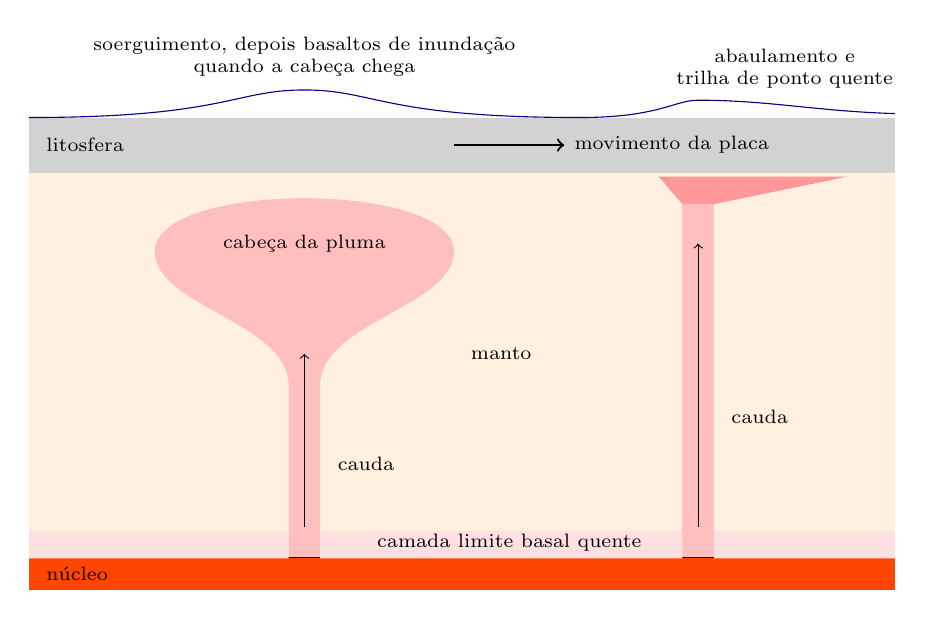
\begin{tikzpicture}[font=\scriptsize, x=1cm, y=1cm]
\fill[orange!12] (0,0) rectangle (11,-5.6);
\fill[gray!35] (0,0) -- (11,0) -- (11,-0.7) -- (0,-0.7) -- cycle;
\fill[red!25] (3.3,-5.6) -- (3.3,-3.4) .. controls (3.3,-2.6) and (1.6,-2.4) .. (1.6,-1.7)
  .. controls (1.6,-0.8) and (5.4,-0.8) .. (5.4,-1.7) .. controls (5.4,-2.4) and (3.7,-2.6) .. (3.7,-3.4) -- (3.7,-5.6) -- cycle;
\fill[red!25] (8.3,-5.6) -- (8.3,-0.75) -- (8.7,-0.75) -- (8.7,-5.6) -- cycle;
\fill[red!40] (8.0,-0.75) -- (8.3,-1.1) -- (8.7,-1.1) -- (10.4,-0.75) -- cycle;
\draw[thick] (0,-5.6) -- (11,-5.6);
\fill[red!45!orange] (0,-5.6) rectangle (11,-6.0);
\fill[red!12] (0,-5.6) rectangle (3.3,-5.25) (3.7,-5.6) rectangle (8.3,-5.25) (8.7,-5.6) rectangle (11,-5.25);
\node[anchor=west] at (0.1,-5.8) {núcleo};
\node at (3.5,-1.6) {cabeça da pluma};
\node[anchor=west] at (3.8,-4.4) {cauda};
\node[anchor=west] at (8.8,-3.8) {cauda};
\node[anchor=west] at (0.1,-0.35) {litosfera};
\node at (6.0,-3.0) {manto};
\draw[->] (3.5,-5.2) -- (3.5,-3.0);
\draw[->] (8.5,-5.2) -- (8.5,-1.6);
\draw[->, thick] (5.4,-0.35) -- (6.8,-0.35) node[right] {movimento da placa};
\draw[blue!50!black] (0,0) .. controls (2.5,0) and (2.6,0.35) .. (3.5,0.35) .. controls (4.4,0.35) and (4.5,0) .. (7,0) .. controls (8,0) and (8.2,0.22) .. (8.5,0.22) .. controls (9.4,0.22) and (10,0.08) .. (11,0.05);
\node[above, align=center] at (3.5,0.4) {soerguimento, depois basaltos de inundação\\quando a cabeça chega};
\node[above, align=center] at (9.6,0.25) {abaulamento e\\trilha de ponto quente};
\node[anchor=west] at (4.3,-5.4) {camada limite basal quente};
\end{tikzpicture}

\par\smallskip{\small Uma pluma jovem (à esquerda) ascende como uma cabeça grande alimentada por uma
cauda fina; quando a cabeça se espalha sob a litosfera, a superfície se eleva e basaltos
de inundação podem entrar em erupção. Uma pluma mais antiga (à direita) é uma cauda sob uma
placa em movimento, alimentando um abaulamento e uma trilha de ponto quente. Fora de
escala.}\label{fig:b3:mantle-convection:plume}
\end{omfigure}

Uma cabeça de pluma é uma esfera de manto de baixa densidade que ascende através do manto viscoso:
a lei de Stokes, $v = 2\Delta\rho\,ga^2/(9\eta)$, fornece sua velocidade em ordem de
grandeza, uma fração de metro por ano para uma cabeça com algumas centenas de quilômetros
de diâmetro (exercício 8), de modo que ela atravessa o manto em milhões de anos.

\section{Ajuste isostático glacial e a viscosidade do manto}\label{sec:b3:mantle-convection:gia}

\begin{definition}[Ajuste isostático glacial, viscosidade do manto]\label{def:b3:mantle-convection:gia}
O \emph{ajuste isostático glacial}\index{ajuste isostático glacial} (GIA)
é a lenta deformação da Terra sólida, e a mudança de seu campo gravitacional
e do nível do mar, à medida que ela retorna ao equilíbrio isostático depois que uma
calota de gelo cresce ou derrete. A \emph{viscosidade do manto}\index{viscosidade do manto}
é a viscosidade efetiva $\eta$ que relaciona a fluência lenta e constante do manto
às tensões que o impulsionam, em escalas de milhares de anos ou mais.
\end{definition}

Quando uma calota de gelo derrete, a depressão que ela deixa está fora do equilíbrio
isostático: sob ela, a pressão do manto é menor do que ao redor, e o manto flui para dentro
para elevar de novo o assoalho. Hoje a costa do golfo de Bótnia
se eleva até \qty{10.3}{mm/yr}, perto de Umeå; a baía de Hudson, cerca de
\qty{10}{mm/yr}, onde o gelo era mais espesso, enquanto a terra ao sul dos Grandes
Lagos afunda de 1 a \qty{2}{mm/yr}, à medida que o abaulamento que o gelo havia empurrado
para cima ao redor dela subsidencia. Nas costas, antigas linhas de praia estão agora acima do mar,
as praias erguidas da caixa de campo abaixo.
% ledger: vestol19:umea, sella07:gia

\begin{theorem}[Relaxação de um semiespaço viscoso]\label{thm:b3:mantle-convection:relaxation}
Uma depressão $w(x, t) = w_m(t)\cos(2\pi x/\lambda)$ da superfície de um
semiespaço de viscosidade uniforme $\eta$ e densidade $\rho$, deixado sem carga,
decai como $w_m(t) = w_m(0)e^{-t/\tau}$ com
\[
  \tau = \frac{4\pi\eta}{\rho g\lambda} .
\]
\end{theorem}

\begin{proof}
Tome-se $z$ para baixo, $k = 2\pi/\lambda$, e procure-se um escoamento de Stokes que decaia
com a profundidade, com velocidade vertical (para baixo) $v = (C + Dkz)e^{-kz}\cos kx$.
A incompressibilidade fornece a velocidade horizontal $u = -(D - C - Dkz)e^{-kz}\sin
kx$. Essas funções satisfazem $\nabla^4 = 0$, como todo escoamento de Stokes em duas
dimensões. A superfície livre não transmite tensão de cisalhamento: $\partial u/\partial
z + \partial v/\partial x = 2k(D - C)\sin kx = 0$ em $z = 0$, logo $D = C$, e
\[
  v = C(1 + kz)e^{-kz}\cos kx,\quad u = Ckze^{-kz}\sin kx,\quad
  p = 2\eta Cke^{-kz}\cos kx,
\]
obtém-se a pressão a partir de $\partial p/\partial x = \eta\nabla^2u = -2\eta
Ck^2e^{-kz}\sin kx$ (e $\partial p/\partial z = \eta\nabla^2v$ se verifica). Na
superfície $\partial v/\partial z = 0$, de modo que a tensão normal ali é $-p$. Sob
uma depressão $w$, o peso da rocha ausente reduz a pressão de $\rho
gw$: $p(0) = -\rho gw$, portanto $2\eta Ck = -\rho gw_m$. A superfície se move com o
fluido: $\mathrm dw_m/\mathrm dt = v(0) = C = -\rho gw_m/(2\eta k)$, cuja
solução decai com $\tau = 2\eta k/(\rho g) = 4\pi\eta/(\rho g\lambda)$.
\end{proof}

\begin{definition}[Tempo de relaxação isostática]\label{def:b3:mantle-convection:relaxation-time}
O \emph{tempo de relaxação isostática}\index{tempo de relaxação isostática} $\tau$ de
uma carga de escala horizontal $\lambda$ é o tempo em que seu afastamento do
equilíbrio isostático decai por um fator $e$.
\end{definition}

Um semiespaço uniforme relaxa depressões largas mais depressa do que as estreitas, e o
escoamento sob uma carga de comprimento de onda $\lambda$ decai com a profundidade como $e^{-kz}$, ao longo de
uma profundidade $\lambda/2\pi$: um grande manto de gelo agita o manto em profundidade, um pequeno lago
apenas o seu topo. Para uma depressão de \qty{3000}{km} de extensão e $\eta =
\qty{e21}{Pa.s}$, com $\rho = \qty{3300}{kg.m^{-3}}$, $\tau = \qty{4.1}{kyr}$
(figura abaixo): após dez mil anos, resta $e^{-2.4} = \qty{9}{\percent}$ da
depressão, e, como $\dot w = -w/\tau$, uma elevação de
\qty{10}{mm/yr} significa que ainda faltam cerca de \qty{40}{m} de subida.

\begin{omfigure}
\begin{tikzpicture}
\begin{groupplot}[group style={group size=1 by 2, vertical sep=2.5cm},
  omrecord, width=0.86\linewidth, height=0.38\linewidth]
\nextgroupplot[xmin=0, xmax=20, ymin=0, ymax=1.05, xlabel={tempo desde o derretimento do gelo (kyr)},
  ylabel={$w_m(t)/w_m(0)$}, title={(a) decaimento de uma depressão de \qty{3000}{km}},
  title style={font=\small}, legend style={font=\scriptsize, at={(0.98,0.97)}, anchor=north east}]
% computed in figdata/bachelor-3/gia_relaxation.py; ledger: mitrovica96:haskell, milne04:bifrost
\addplot[red!70!black, thick, densely dashed] table[x=t, y=f20] {figdata/out/bachelor-3-gia_relaxation-decay.dat};
\addlegendentry{$\eta = \qty{e20}{Pa.s}$}
\addplot[omDef, thick] table[x=t, y=f21] {figdata/out/bachelor-3-gia_relaxation-decay.dat};
\addlegendentry{$\eta = \qty{e21}{Pa.s}$}
\addplot[black, thick, densely dotted] table[x=t, y=f22] {figdata/out/bachelor-3-gia_relaxation-decay.dat};
\addlegendentry{$\eta = \qty{e22}{Pa.s}$}
\nextgroupplot[xmode=log, ymode=log, xmin=100, xmax=1e4, ymin=0.01, ymax=1000,
  xlabel={comprimento de onda $\lambda$ (km)}, ylabel={$\tau$ (kyr)},
  title={(b) tempo de relaxação em função do comprimento de onda}, title style={font=\small}]
\addplot[red!70!black, thick, densely dashed] table[x=lam, y=t20] {figdata/out/bachelor-3-gia_relaxation-tau.dat};
\addplot[omDef, thick] table[x=lam, y=t21] {figdata/out/bachelor-3-gia_relaxation-tau.dat};
\addplot[black, thick, densely dotted] table[x=lam, y=t22] {figdata/out/bachelor-3-gia_relaxation-tau.dat};
\end{groupplot}
\end{tikzpicture}

\par\smallskip{\small Relaxação de um semiespaço viscoso uniforme ($\rho =
\qty{3300}{kg.m^{-3}}$, $g = \qty{9.8}{m.s^{-2}}$) para três viscosidades. (a) A
fração da depressão que resta ao longo do tempo. (b) O tempo de relaxação
$4\pi\eta/(\rho g\lambda)$, mais longo para cargas estreitas.}\label{fig:b3:mantle-convection:gia}
\end{omfigure}

O manto real não é uniforme, e seu rebote é lido com modelos que o estratificam
e acrescentam uma litosfera elástica, que sustenta cargas estreitas por flexura. A
primeira estimativa, a partir do rebote da Fennoscândia, deu \qty{e21}{Pa.s}, e o
decaimento do levantamento no rio Angerman, na Suécia, e em Richmond Gulf, na baía de Hudson,
fornece uma média de 0.65 a \qty{1.1e21}{Pa.s}, desde a base da
litosfera até cerca de \qty{1400}{km}, sendo o manto superior cerca de dez vezes
menos viscoso do que o inferior. Inversões das taxas de levantamento por GNSS da
Fennoscândia dão \omterm{def:b3:mantle-convection:gia}{viscosidades do manto} superior de \num{5e20} a \qty{e21}{Pa.s}
em um estudo e de \num{3.4e20} a \qty{5.0e20}{Pa.s} em outro, \omterm{def:b3:mantle-convection:gia}{viscosidades do manto} inferior
de \num{5e21} a \qty{5e22}{Pa.s}, e uma litosfera com espessura de 93 a
\qty{110}{km}. As estimativas diferem por fatores de dois ou três, mas concordam
na ordem de grandeza e no aumento com a profundidade.
% ledger: mitrovica96:haskell, milne04:bifrost, zhao12:fenno

\begin{definition}[Tempo de Maxwell]\label{def:b3:mantle-convection:maxwell}
O \emph{tempo de Maxwell}\index{tempo de Maxwell} de um material de viscosidade $\eta$
e módulo de cisalhamento $\mu$ é $\tau_M = \eta/\mu$: cargas aplicadas por muito menos que
$\tau_M$ encontram um sólido elástico, cargas aplicadas por muito mais tempo encontram um fluido viscoso.
\end{definition}

Com $\mu = \rho v_S^2 = \qty{7.7e10}{Pa}$ a \qty{300}{km} no PREM e $\eta =
\qty{e21}{Pa.s}$, $\tau_M = \qty{1.3e10}{s}$, cerca de quatrocentos anos. Uma
onda sísmica, que dura segundos, atravessa um manto elástico; uma era glacial e
a convecção deformam um fluido. A mesma rocha é as duas coisas, dependendo de
quanto tempo é empurrada.
% ledger: data:prem

\begin{inthefield}[Praias erguidas]
\begin{minipage}[t]{0.55\linewidth}\vspace{0pt}
Nas costas de terras outrora glaciadas, um geomorfólogo encontra o trabalho antigo do mar
encalhado no interior: cordões de seixos arredondados, entalhes e plataformas planas
escavadas pelas ondas, agora situados acima do alcance das marés mais altas de hoje,
por vezes em uma escadaria de vários níveis. Cada nível foi uma linha de costa
quando o mar ali se encontrava; desde então a terra se elevou. Conchas e madeira flutuante nas
praias antigas são datadas por radiocarbono, e as alturas dos níveis datados,
nivelados a um marco de referência, fornecem o levantamento em função do tempo. Traçada ao longo de uma costa,
uma linha de costa antiga revela-se inclinada, mais alta onde o gelo era mais espesso: a
inclinação mapeia a forma do rebote.
\end{minipage}\hfill
\begin{minipage}[t]{0.42\linewidth}\vspace{0pt}
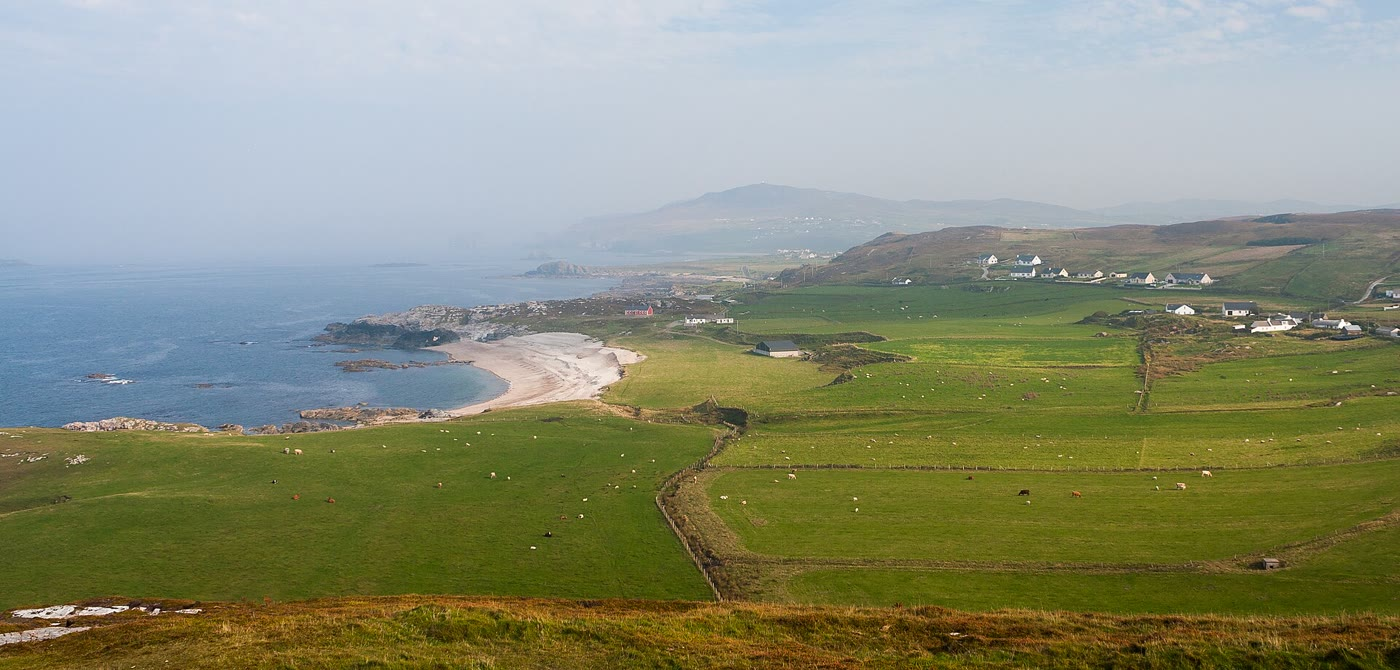
\includegraphics[width=\linewidth]{images/book5/b3-raised-beach-malin.jpg}

{\scriptsize As praias erguidas de Ballyhillin, Malin Head, no norte da
Irlanda: cordões de seixos de antigas linhas de costa elevadas acima do mar à medida que a terra se soergueu
após o derretimento de seu manto de gelo. Foto A.~F.~Borchert, CC BY-SA 4.0.}
\end{minipage}
\end{inthefield}
% ledger: photo:b3-raised-beach

\section{Convecção de todo o manto e sua estrutura profunda}

O manto convecta em uma só camada ou em duas, acima e abaixo da
descontinuidade de \qty{670}{km}? A tomografia (veja o \cref{ch:b3:seismology-imaging})
responde em parte: algumas lajes se achatam acima da descontinuidade, outras mergulham
através dela no manto inferior, de modo que material a atravessa e as duas camadas não são
isoladas uma da outra. O aumento da viscosidade com a profundidade faz o manto
inferior fluir mais lentamente, e as lajes desaceleram e se espessam ao entrar nele.

Na base do manto, a tomografia mostra duas grandes regiões de baixa velocidade de onda S,
sob a África e sob o Pacífico, as grandes províncias de baixa velocidade de cisalhamento
(LLSVPs). Elas são provavelmente quimicamente distintas do manto acima
delas e mais densas, são pilhas e não plumas quentes. As grandes províncias ígneas e
os kimberlitos das últimas algumas centenas de milhões de anos entraram em erupção sobretudo acima de suas
margens, como se plumas subissem das bordas das pilhas, onde a camada limite quente
da base do manto é varrida contra elas.
% ledger: st12:llsvp

\section*{Exercícios}

\begin{exercise}[$\star$]\label{exo:b3:mantle-convection:1}
Calcule o \omterm{def:b3:mantle-convection:rayleigh}{número de Rayleigh} de uma camada do manto superior com \qty{670}{km} de espessura, com
$\rho = \qty{3500}{kg.m^{-3}}$, $g = \qty{9.9}{m.s^{-2}}$, $\alpha =
\qty{3e-5}{K^{-1}}$, $\Delta T = \qty{1000}{K}$, $\kappa =
\qty{e-6}{m^2.s^{-1}}$ e $\eta = \qty{5e20}{Pa.s}$. Quantas vezes ele supera
o valor crítico, para contornos de deslizamento livre?
\end{exercise}

\begin{exercise}[$\star$]\label{exo:b3:mantle-convection:2}
Calcule o \omterm{def:b3:mantle-convection:maxwell}{tempo de Maxwell} de um manto de viscosidade \qty{e21}{Pa.s} e módulo de cisalhamento
de \qty{7.7e10}{Pa}, em anos. O manto responde de forma elástica ou
viscosa à maré terrestre semidiurna, ao derretimento de um manto de gelo e à
deformação causada pelo afundamento de uma laje?
\end{exercise}

\begin{exercise}[$\star$]\label{exo:b3:mantle-convection:3}
Com $\eta = \qty{e21}{Pa.s}$, $\rho = \qty{3300}{kg.m^{-3}}$ e $g =
\qty{9.8}{m.s^{-2}}$, calcule o tempo de relaxação de um semiespaço uniforme para
cargas de comprimento de onda 1000 e \qty{3000}{km}. Qual delas se recupera mais rapidamente?
\end{exercise}

\begin{exercise}[$\star$]\label{exo:b3:mantle-convection:4}
Com $g = \qty{9.8}{m.s^{-2}}$, $\rho_m = \qty{3300}{kg.m^{-3}}$, $\rho_w =
\qty{1030}{kg.m^{-3}}$, $\alpha = \qty{3.1e-5}{K^{-1}}$, $T_m - T_0 =
\qty{1450}{K}$, $\kappa = \qty{0.8e-6}{m^2.s^{-1}}$ e \qty{1}{Myr} $=
\qty{3.156e13}{s}$, calcule a \omterm{prop:b3:mantle-convection:ridge-push}{força de empurrão da dorsal} aos \qty{50}{Myr}. Quantas vezes
ela é menor que a tração da laje de \qty{4.6e13}{N.m^{-1}}?
\end{exercise}

\begin{exercise}[$\star\star$]\label{exo:b3:mantle-convection:5}
Uma porção de manto de \qty{10}{km} de largura, \qty{300}{K} mais quente que seus
arredores, sobe com velocidade $\rho g\alpha\Delta Td^2/\eta$ (tome $\rho =
\qty{3300}{kg.m^{-3}}$, $g = \qty{9.8}{m.s^{-2}}$, $\alpha = \qty{3e-5}{K^{-1}}$,
$\eta = \qty{e21}{Pa.s}$, $\kappa = \qty{e-6}{m^2.s^{-1}}$). (a) Calcule seu
tempo de ascensão ao atravessar o próprio tamanho e seu tempo de difusão $d^2/\kappa$, e mostre
que a razão entre eles é seu \omterm{def:b3:mantle-convection:rayleigh}{número de Rayleigh}. (b) Ela sobe ou se resfria primeiro? (c)
Qual deve ser o tamanho dela para que seu \omterm{def:b3:mantle-convection:rayleigh}{número de Rayleigh} atinja 657.5?
\end{exercise}

\begin{exercise}[$\star\star$]\label{exo:b3:mantle-convection:6}
Para uma camada de \qty{2891}{km} de profundidade com $\mathrm{Ra} = \num{e7}$, com $\kappa =
\qty{e-6}{m^2.s^{-1}}$, $k = \qty{3.1}{W.m^{-1}.K^{-1}}$, $\Delta T =
\qty{1450}{K}$ e $\mathrm{Ra}_c = 657.5$, calcule a espessura da camada limite,
o \omterm{def:b3:mantle-convection:nusselt}{número de Nusselt}, a escala de velocidade em \unit{cm/yr} e o
fluxo de calor.
\end{exercise}

\begin{exercise}[$\star\star$]\label{exo:b3:mantle-convection:7}
Uma elevação de ponto quente fictícia tem área de seção transversal de \qty{8e8}{m^2} através
da trilha, e a placa acima se move a \qty{9}{cm/yr}. Com $\rho_m - \rho_w =
\qty{2270}{kg.m^{-3}}$, calcule seu fluxo de empuxo e seu fluxo de calor com $c_p =
\qty{1170}{J.kg^{-1}.K^{-1}}$ e $\alpha = \qty{3.1e-5}{K^{-1}}$. Qual fração
do total terrestre de \qty{46.7}{TW} ela representa?
\end{exercise}

\begin{exercise}[$\star\star$]\label{exo:b3:mantle-convection:8}
Uma cabeça de pluma de raio \qty{400}{km}, mais leve que o manto em
\qty{30}{kg.m^{-3}}, sobe através de um manto de viscosidade \qty{e21}{Pa.s}. Com
a lei de Stokes, calcule sua velocidade em \unit{m/yr} e o tempo necessário para subir
\qty{2000}{km}.
\end{exercise}

\begin{exercise}[$\star\star$]\label{exo:b3:mantle-convection:9}
Uma região foi deprimida em \qty{300}{m} quando seu gelo derreteu, há \qty{10}{kyr},
e relaxa com $\tau = \qty{4.4}{kyr}$. Calcule a depressão remanescente hoje e
a taxa atual de soerguimento. Compare com a de \qty{10.3}{mm/yr} medida perto de
Umeå.
\end{exercise}

\begin{exercise}[$\star\star\star$]\label{exo:b3:mantle-convection:10}
(a) A partir da expressão de $F_{rp}$ na demonstração
da \cref{prop:b3:mantle-convection:ridge-push}, mostre que o primeiro termo,
$\tfrac12(\rho_m - \rho_w)gw^2$, é o segundo termo do colchete. (b) Mostre que
$\int_0^\infty x\operatorname{erfc}x\,\mathrm dx = 1/4$, integrando por partes.
(c) Com os valores do exercício 4, calcule os dois termos aos \qty{100}{Myr}.
\end{exercise}

\begin{exercise}[$\star\star\star$]\label{exo:b3:mantle-convection:11}
Mostre que $f(k) = (\pi^2 + k^2)^3/k^2$ é mínima em $k = \pi/\sqrt2$, onde
ela vale $27\pi^4/4$. Deduza a largura de um par de células de convecção no início
da convecção, em unidades de $d$, e a largura de uma célula.
\end{exercise}

\begin{exercise}[$\star\star\star$]\label{exo:b3:mantle-convection:12}
Uma placa de \qty{6000}{km} de comprimento se move a \qty{6}{cm/yr} sobre uma camada do manto
de \qty{150}{km} de espessura e viscosidade \qty{e20}{Pa.s}, cuja base está em repouso. (a)
Calcule o \omterm{def:b3:mantle-convection:basal-drag}{arrasto basal} em \unit{MPa} e a força de arrasto por unidade de comprimento da placa.
(b) Compare com um empurrão da dorsal de \qty{3.8e12}{N.m^{-1}} e uma tração da laje de
\qty{4.6e13}{N.m^{-1}}. (c) Se um décimo da tração da laje chega à placa,
com que velocidade o arrasto equilibra as forças motrizes?
\end{exercise}

\section{Problema: Rebote do lago Ardo}

\begin{problem}[{Problema de fim de semana --- o rebote de uma bacia lacustre inventada,
a viscosidade do manto sob ela e a convecção que tal viscosidade
possibilita}]
\label{pb:b3:mantle-convection:1}
% values: calc/ch06.py; gia_relaxation.py, convection_scaling.py
O lago Ardo, um lago inventado, ocupava uma bacia de \qty{250}{km} de largura, represada por um
manto de gelo, e manteve-se com \qty{300}{m} de profundidade durante cerca de cinquenta mil anos. Catorze
mil anos atrás a barragem de gelo rompeu-se e o lago drenou em poucas semanas. A sua
linha de praia mais alta, horizontal quando se formou, está agora inclinada; as linhas de praia datadas
dos pequenos lagos que restaram na bacia fornecem o soerguimento do centro desde a
drenagem, em relação à borda, que quase não se moveu:

\smallskip
\begin{center}\small
\begin{tabular}{lcccccc}
\hline
tempo desde a drenagem (kyr) & 1 & 2 & 4 & 6 & 9 & 14\\
soerguimento do centro (m) & 11.5 & 21.6 & 38.0 & 50.5 & 64.0 & 77.2\\
\hline
\end{tabular}
\end{center}
\smallskip

Considere $\rho_w = \qty{1000}{kg.m^{-3}}$, $\rho_m = \qty{3300}{kg.m^{-3}}$, $g =
\qty{9.8}{m.s^{-2}}$, \qty{1}{yr} $= \qty{3.156e7}{s}$, e trate o manto como
um semiespaço viscoso uniforme.

\medskip\noindent\textbf{Parte I --- A carga.}
\begin{enumerate}
  \item Calcule a pressão do lago sobre o seu fundo.
  \item Calcule a depressão do fundo em equilíbrio isostático e diga
        por que a densidade do manto, e não a da crosta, aparece nela.
  \item Considerando o lago como um disco, calcule a massa de sua água.
  \item Explique por que a linha de praia mais alta está agora inclinada e calcule sua
        inclinação média da borda até o centro, em metros por quilômetro.
  \item A depressão é tratada como um único harmônico cuja metade deprimida, de
        $-\lambda/4$ a $\lambda/4$, abrange o lago. Dê $\lambda$ e $k =
        2\pi/\lambda$.
  \item Em que profundidade o escoamento sob tal carga decai pelo fator
        $e$?
\end{enumerate}

\medskip\noindent\textbf{Parte II --- O tempo de relaxação.}
\begin{enumerate}[resume]
  \item Supondo que o lago tivesse atingido o equilíbrio, calcule a depressão restante
        em cada data da tabela.
  \item Mostre que, se a depressão decai exponencialmente, seu logaritmo cai
        linearmente com o tempo.
  \item Calcule $\tau$ a partir das datas de 1 e \qty{14}{kyr}.
  \item Preveja o soerguimento em \qty{6}{kyr} com esse $\tau$ e compare com a
        tabela.
  \item Calcule a depressão restante hoje e a taxa atual de soerguimento do
        centro, em \unit{mm/yr}.
  \item Quanto soerguimento ainda falta?
  \item Em quantos anos mais a taxa de soerguimento cairá abaixo de
        \qty{0.5}{mm/yr}?
\end{enumerate}

\medskip\noindent\textbf{Parte III --- A viscosidade.}
\begin{enumerate}[resume]
  \item Calcule a viscosidade do semiespaço a partir de $\tau$.
  \item Compare-a com as \omterm{def:b3:mantle-convection:gia}{viscosidades do manto} superior de \num{3.4e20} a
        \qty{1e21}{Pa.s} encontradas sob a Fennoscândia. Que parte do manto
        o rebote do lago Ardo amostra?
  \item Com essa viscosidade, calcule o tempo de relaxação de uma carga
        de \qty{3000}{km} de comprimento de onda. Por que um manto de gelo real desse
        tamanho relaxaria mais lentamente do que isto?
  \item O que faz uma litosfera elástica, desprezada aqui, com o rebote de uma
        carga de apenas \qty{250}{km} de largura?
  \item Calcule o \omterm{def:b3:mantle-convection:maxwell}{tempo de Maxwell} do manto com $\mu = \qty{7.7e10}{Pa}$,
        e diga se um modelo viscoso era justificado.
  \item Verifique a hipótese da questão 7: que fração da depressão de equilíbrio
        foi atingida enquanto o lago existiu?
  \item De quanto mudaria $\log_{10}\eta$ se $\lambda$ fosse tomado como
        \qty{250}{km}?
\end{enumerate}

\medskip\noindent\textbf{Parte IV --- Convecção.} Considere uma camada do manto superior
de \qty{670}{km} de profundidade, com $\rho = \qty{3700}{kg.m^{-3}}$, $g =
\qty{9.9}{m.s^{-2}}$, $\alpha = \qty{3.1e-5}{K^{-1}}$, $\Delta T =
\qty{1450}{K}$, $\kappa = \qty{e-6}{m^2.s^{-1}}$, $k = \qty{3.1}{W.m^{-1}.K^{-1}}$
e a viscosidade da Parte III.
\begin{enumerate}[resume]
  \item Calcule o \omterm{def:b3:mantle-convection:rayleigh}{número de Rayleigh} da camada.
  \item Quantas vezes ele supera o valor crítico ($\mathrm{Ra}_c = 657.5$)?
  \item Calcule a espessura da camada limite e o \omterm{def:b3:mantle-convection:nusselt}{número de Nusselt}.
  \item Calcule a escala de velocidade em \unit{cm/yr} e compare com as velocidades
        das placas, de 1 a \qty{7.5}{cm/yr}.
  \item Calcule o fluxo de calor e dê duas razões pelas quais ele fica aquém da
        média da Terra, \qty{92}{mW.m^{-2}}.
  \item Dê a \omterm{def:b3:mantle-convection:gia}{viscosidade do manto} superior sob o lago Ardo como $\log_{10}$ de
        $\eta$ em \unit{Pa.s}.
\end{enumerate}
\end{problem}
